\section{Visitors}
\label{section:visitors}
Since patterns, term-templates and top-level forms require analysis or transformations applied to them, visitors for each \texttt{TermTemplate}, \texttt{Pattern} and \texttt{TopLevelForm} are provided, as seen in Figure \ref{class-diagram-visitors}. 

In other programming languages \texttt{Visitor} design pattern would require each \texttt{TermTemplate}, \texttt{Pattern} or \texttt{TopLevelForm} class to implement \texttt{accept} method with \texttt{Visitor} passed as parameter. However, since Python is a dynamic language, meaning it is possible to invoke methods given their names as strings. \texttt{\_visit} method does exactly that - it looks up type-name of passed element, constructs the string, attempts to retrieve the method, and calls it. For example, given \texttt{PatternSequence} instance, resulting method name would be \texttt{\_visitPatternSequence}.

The only method of interest left is \texttt{run}. It is expected to be overridden by each transformation or analysis pass.  Since patterns used in \texttt{define-language} form require different treatment, \texttt{run} implementation may contain iteration logic over \texttt{define-language}, calling \texttt{\_visit} on each pattern. 

\section{\texttt{Annotatable} Class}

When applying transformations/analyses passes to top-level forms, patterns, and term-template, additional information needs to be stored pertaining to those elements. One more obvious idea is to store those bits of information in a seperate hash-map or dictionary, with \texttt{TermTemplate}, \texttt{Pattern} or \texttt{TopLevelForm} elements acting as keys. Unfrtunately, the problem with this approach is that transformation passes may completely replace these elements, making keys in the dictionary invalid.

The solution PyPltRedex employs is storing these bits of information directly in the nodes. \texttt{TermTemplate}, \texttt{Pattern}, and \texttt{TopLevelForm} are subclasses of \texttt{Annotatable} class, class diagram of which can be seen in Figure \ref{class-diagram-visitors}.

Python's dynamicity is leveraged to store arbitrary infromation in the dictionary with \texttt{str} instances acting as keys. \texttt{addmetadata} adds data to the dictionary, \texttt{getmetadata} retrieves it from the dictionary. \texttt{removemetadata} removes key-value pair from the dictionary. \texttt{copymetadatafrom} makes a shallow copy of the dictionary of the provided element, in case if the element is being replaced with something else.

\begin{figure}[ht]
	\centering
	\makebox[\textwidth][c] { 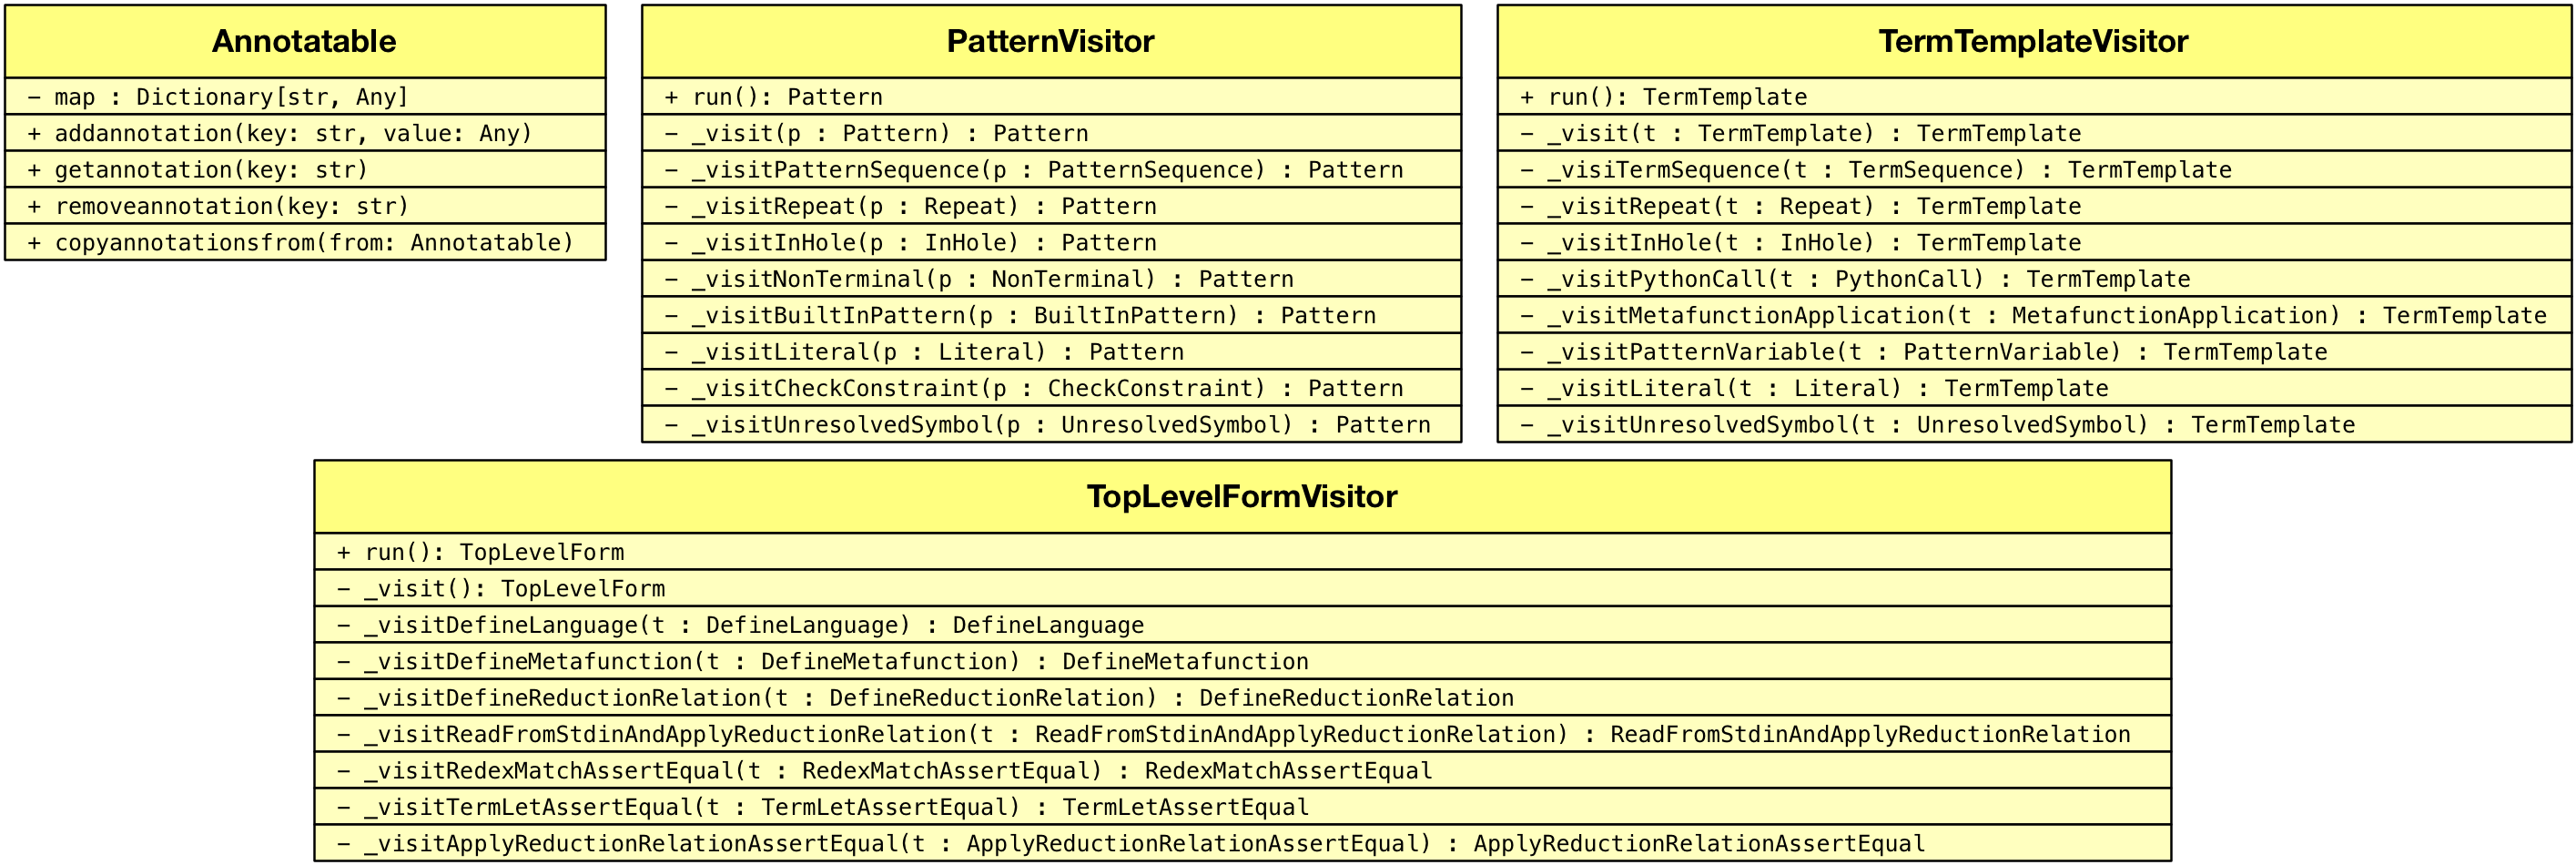
\includegraphics[scale=0.18]{class-diagram-visitors.png} }
	\caption{Representation of visitors and \texttt{Annotatable} class.}
\label{class-diagram-visitors}
\end{figure}

\FloatBarrier
